\documentclass{article}
\usepackage[final]{neurips_2019}

\usepackage[utf8]{inputenc} % allow utf-8 input
\usepackage[T1]{fontenc}    % use 8-bit T1 fonts
\usepackage{hyperref}       % hyperlinks
\usepackage{url}            % simple URL typesetting
\usepackage{booktabs}       % professional-quality tables
\usepackage{amsfonts}       % blackboard math symbols
\usepackage{nicefrac}       % compact symbols for 1/2, etc.
\usepackage{microtype}      % microtypography
\usepackage{amsmath}
\usepackage{graphicx}
\usepackage{subfigure}
\title{Exeriese 3}

\author{%
  Lan Zhang\\
  954517477\\
}

\begin{document}
\maketitle

\section{Problem 1}

Solved on 11/02/2019. The seed I used in bellowing experiments is 2612. 



\subsection{Batch Normalization}
I implement batch normalization after the convontional layer. Figure \ref{fig:bn} is the performance of the model with and without batch normalization. With batch normalization, the model can converge faster.

Then, I tried to compare my implements of batch normalization with tensorflow's implements. At first, I didn't add trainable variables and calculate their gredients. The results of tensorflow' batch normalization layer is highly different from mine. After applying gredients, Figure \ref{fig:com_bn} is the performace of my batch normalization and tensorflow's batch normalization. The difference of two implement is quite small(less than 0.01). I extracted comparable parameters of two batch normalization layer -- gamma and  beta, and summerized their differences shown as Figure \ref{fig:com_bn_param}. The differences of parameters are gradually increase. I think the implements of tensorflow is more complex and may have other mechanism that lend the differences.

\begin{figure}[h]
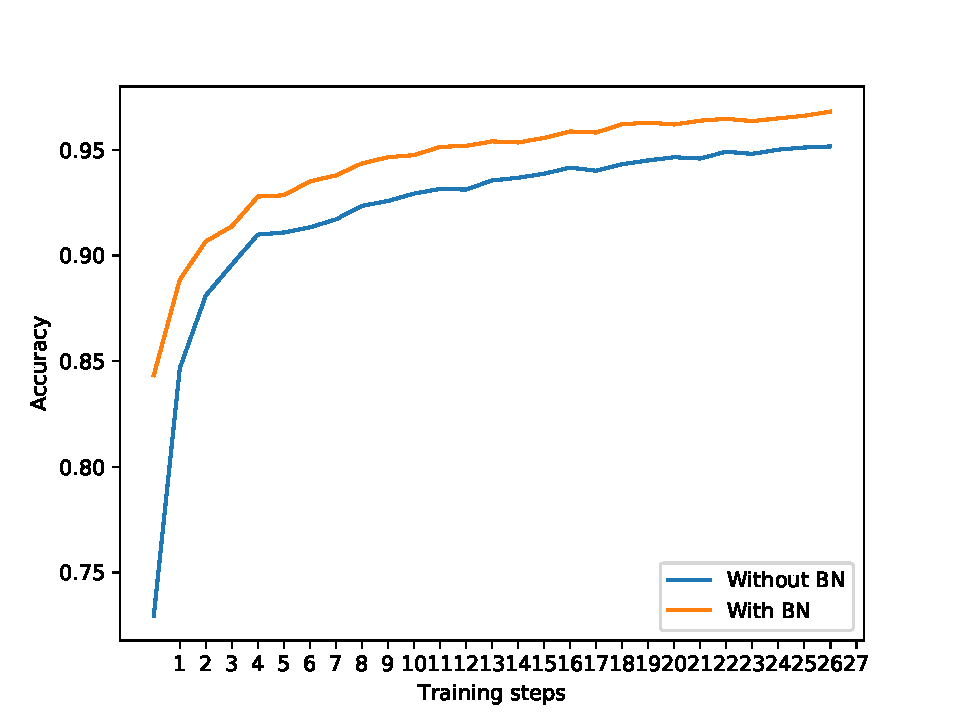
\includegraphics[scale=0.8]{img/bn1.pdf}
\caption{Performance of batch normalization on test dataset.}
\label{fig:bn}
\end{figure}

\begin{figure}[h]
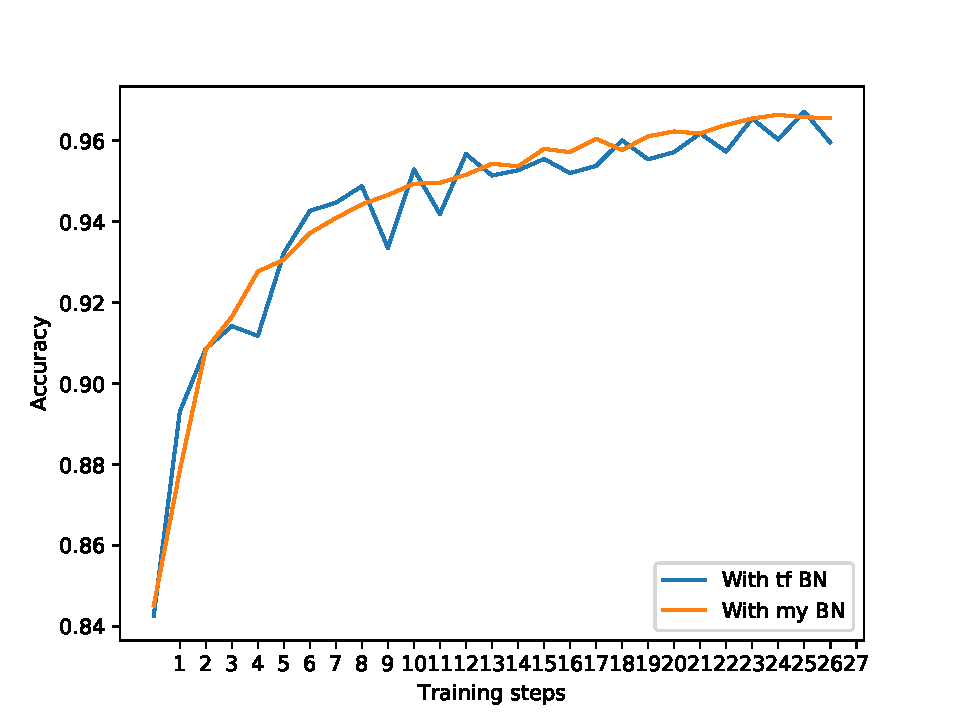
\includegraphics[scale=0.8]{img/com_BN1.pdf}
\caption{Compare my implements of batch normalization with tensorflow's implements}
\label{fig:com_bn}
\end{figure}

\begin{figure}[h]
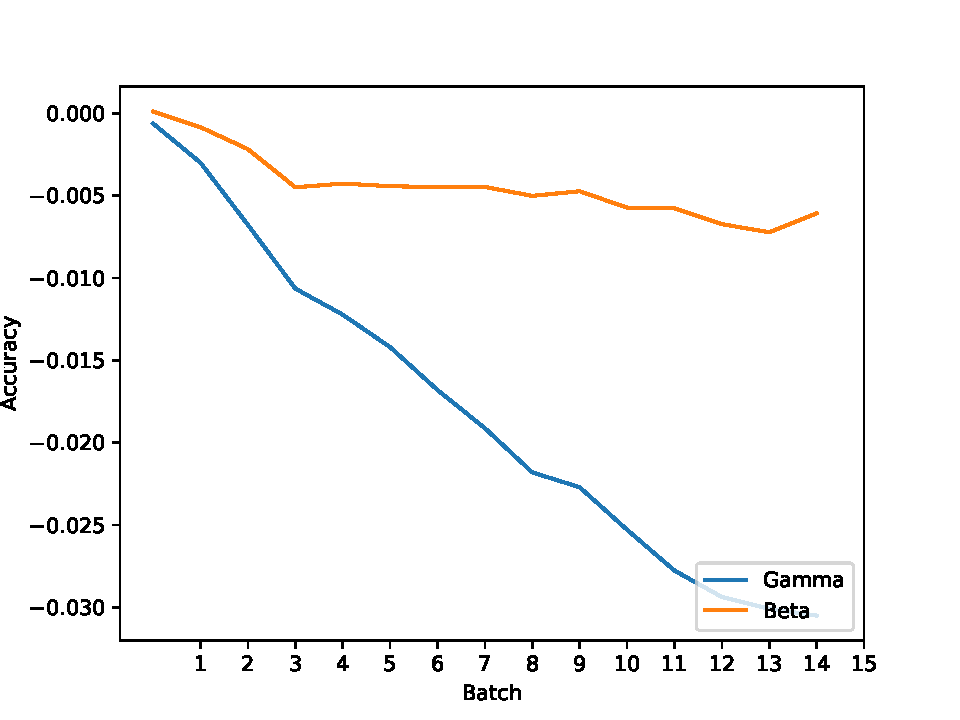
\includegraphics[scale=0.8]{img/com_param_BN.pdf}
\caption{Compare parameters difference of batch normalization}
\label{fig:com_bn_param}
\end{figure}

\subsection{Layer Normalization}
Layer normalization is implemented after the convontional layer. Figure \ref{fig:ln} is the performance of the model with and without layer normalization. %why layer normalization

Then, I compared my implements of layer normalization with tensorflow's implements. After applying gredients, Figure \ref{fig:com_ln} is the performace of my layer normalization and tensorflow's layer normalization. I guess the reason why my layer normalization is better than tensorflow's is **. I extracted comparable parameters of two layer normalization -- gamma and  beta, and summerized their differences shown as Figure \ref{fig:com_ln_param} .

\begin{figure}[h]
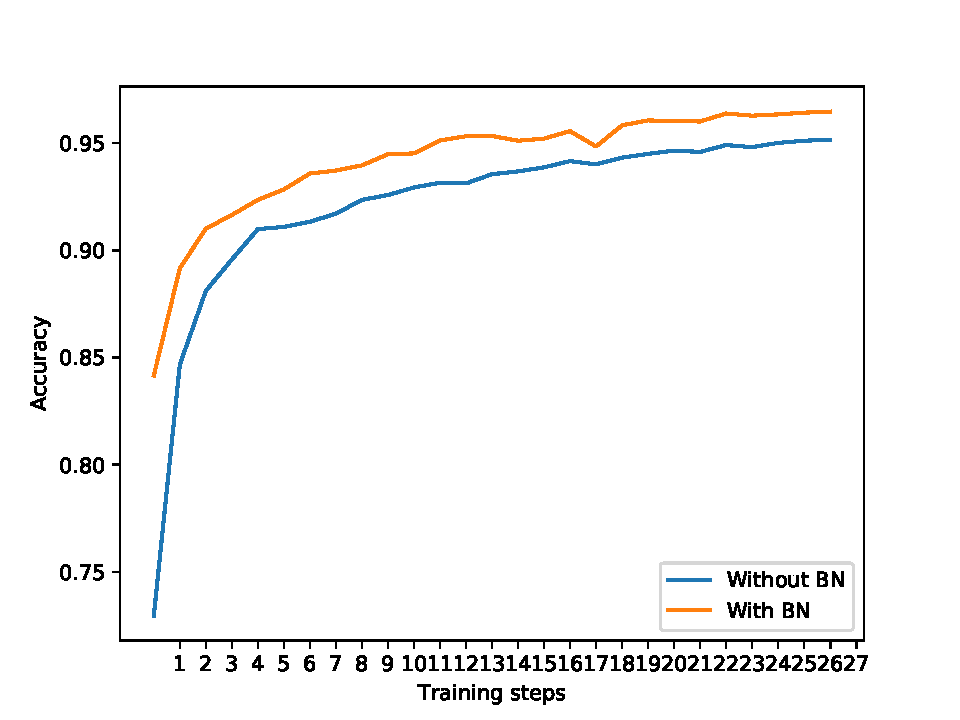
\includegraphics[scale=0.8]{img/ln1.pdf}
\caption{Performance of layer normalization on test dataset.}
\label{fig:ln}
\end{figure}

\begin{figure}[h]
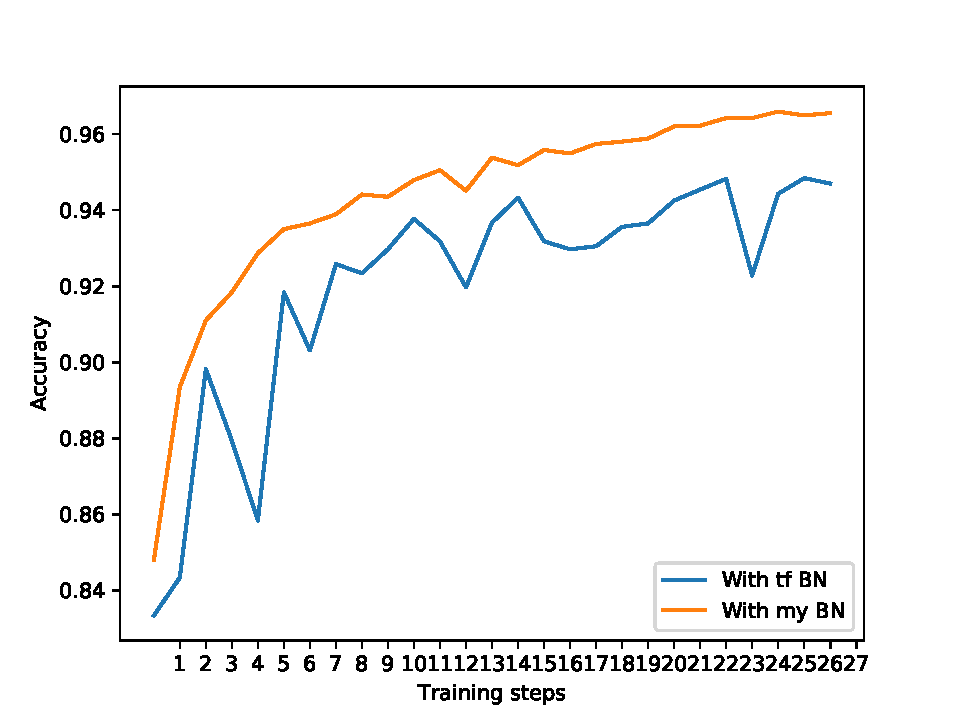
\includegraphics[scale=0.8]{img/com_LN1.pdf}
\caption{Compare my implements of layer normalization with tensorflow's implements}
\label{fig:com_ln}
\end{figure}

\begin{figure}[h]
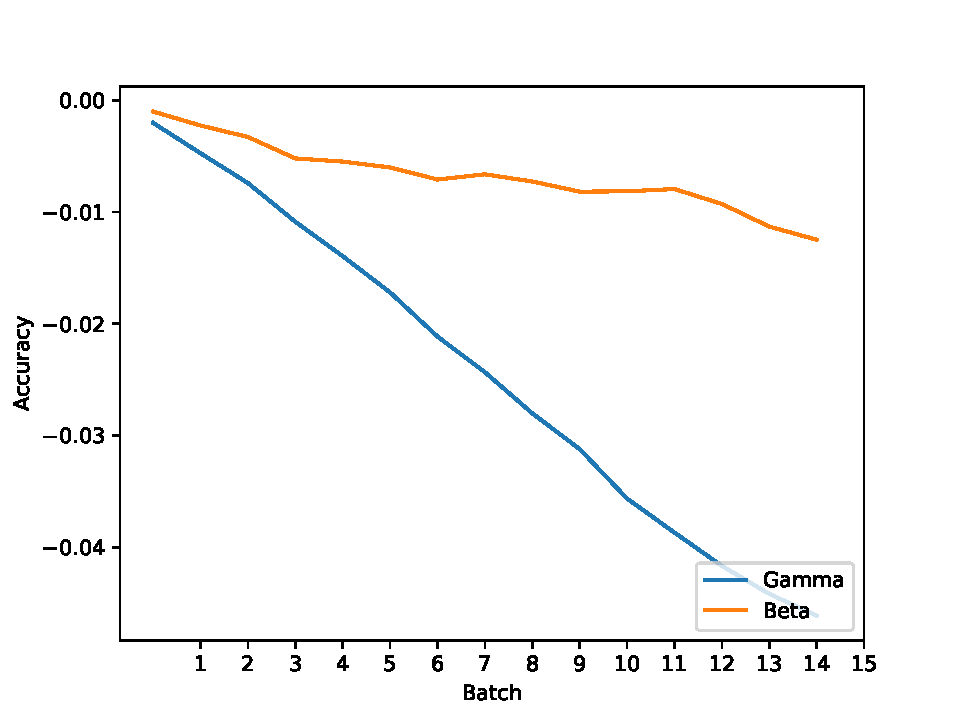
\includegraphics[scale=0.8]{img/com_param_LN.pdf}
\caption{Compare my implements of layer normalization with tensorflow's implements}
\label{fig:com_ln_param}
\end{figure}

\subsection{Weight Normalization}
Weight normalization is implemented before the convontional layer. Figure \ref{fig:wn} is the performance of the model with and without weight normalization. %why layer normalization

\subsection{The performance of different normalization}

\end{document}
